\section{A Brief Review of RSC Codes}
\label{sec2}
The output bits of an RSC code are generated using the feedforward and feedback connections of shift registers determined by its generator function. The generator function may be written in polynomial notation as $\Big[1 ~\frac{f(x)}{g(x)}\Big]$, where $1$ yields the systematic (input) bits  of the output while the parity check bits of the output are specified by  $f(x)$ and $g(x)$ that represent the feedforward and feedback connections of the shift registers respectively. 
%The minimum distance ($d_{\text{min}}$) of the RSC code determines its error-correcting capability. With the aid of the distance spectrum, it is possible to determine $d_{\text{min}}$ as well as its multiplicity. The most common way to find the distance spectrum is via the transfer function of the RSC code. The transfer function enumerates all the paths that diverge from and then return to the initial state \cite{ref3}, \textit{i.e.} the RTZ inputs. In other words, the distance spectrum provides information about the number of codewords of weight $d$ generated by an RTZ input of weight $w$. 

For a given RSC code, the distance spectrum provides information concerning the multiplicity of a codeword for a fixed weight and it is an effective tool to evaluate its error-correcting capability.
Since higher-weight codewords have very little effect on its overall error-correcting capability, it is not unusual to use a partial distance spectrum, where the largest codeword weight value is set to $d_{\text{max}}$. 

The distance spectrum of the RSC code can be obtained from its transfer function, denoted by $$T(Y,X)=\sum_{d=0}^{\infty}\sum_{w=0}^{\infty} a(d,w)Y^dX^w$$ where $a(d,w)$ is the number of codewords of weight $d$ generated by an input message of weight $w$. The transfer function enumerates all the paths that diverge from and then return to the initial state \cite{ref3}, \textit{i.e.} the \textit{return-to-zero} (RTZ) inputs.
The complexity involved in deriving the transfer function increases as the number of states of the RSC code increases and other methods such as Mason's Rule \cite{ref3} have to be used. 
%Also to obtain the distance spectrum requires an extra division operation. In the case of interleaver design for turbo codes, this method for generating the distance spectrum is not particularly useful. This is because it reveals no extra details with respect to the structure of the RTZ inputs. 
%Next, we present our novel method, whose complexity is independent of the number of states in the RSC code. As an added bonus, information regarding the structure of the RTZ inputs can be obtained using this method.

%\begin{figure}[h]
%\centering
%		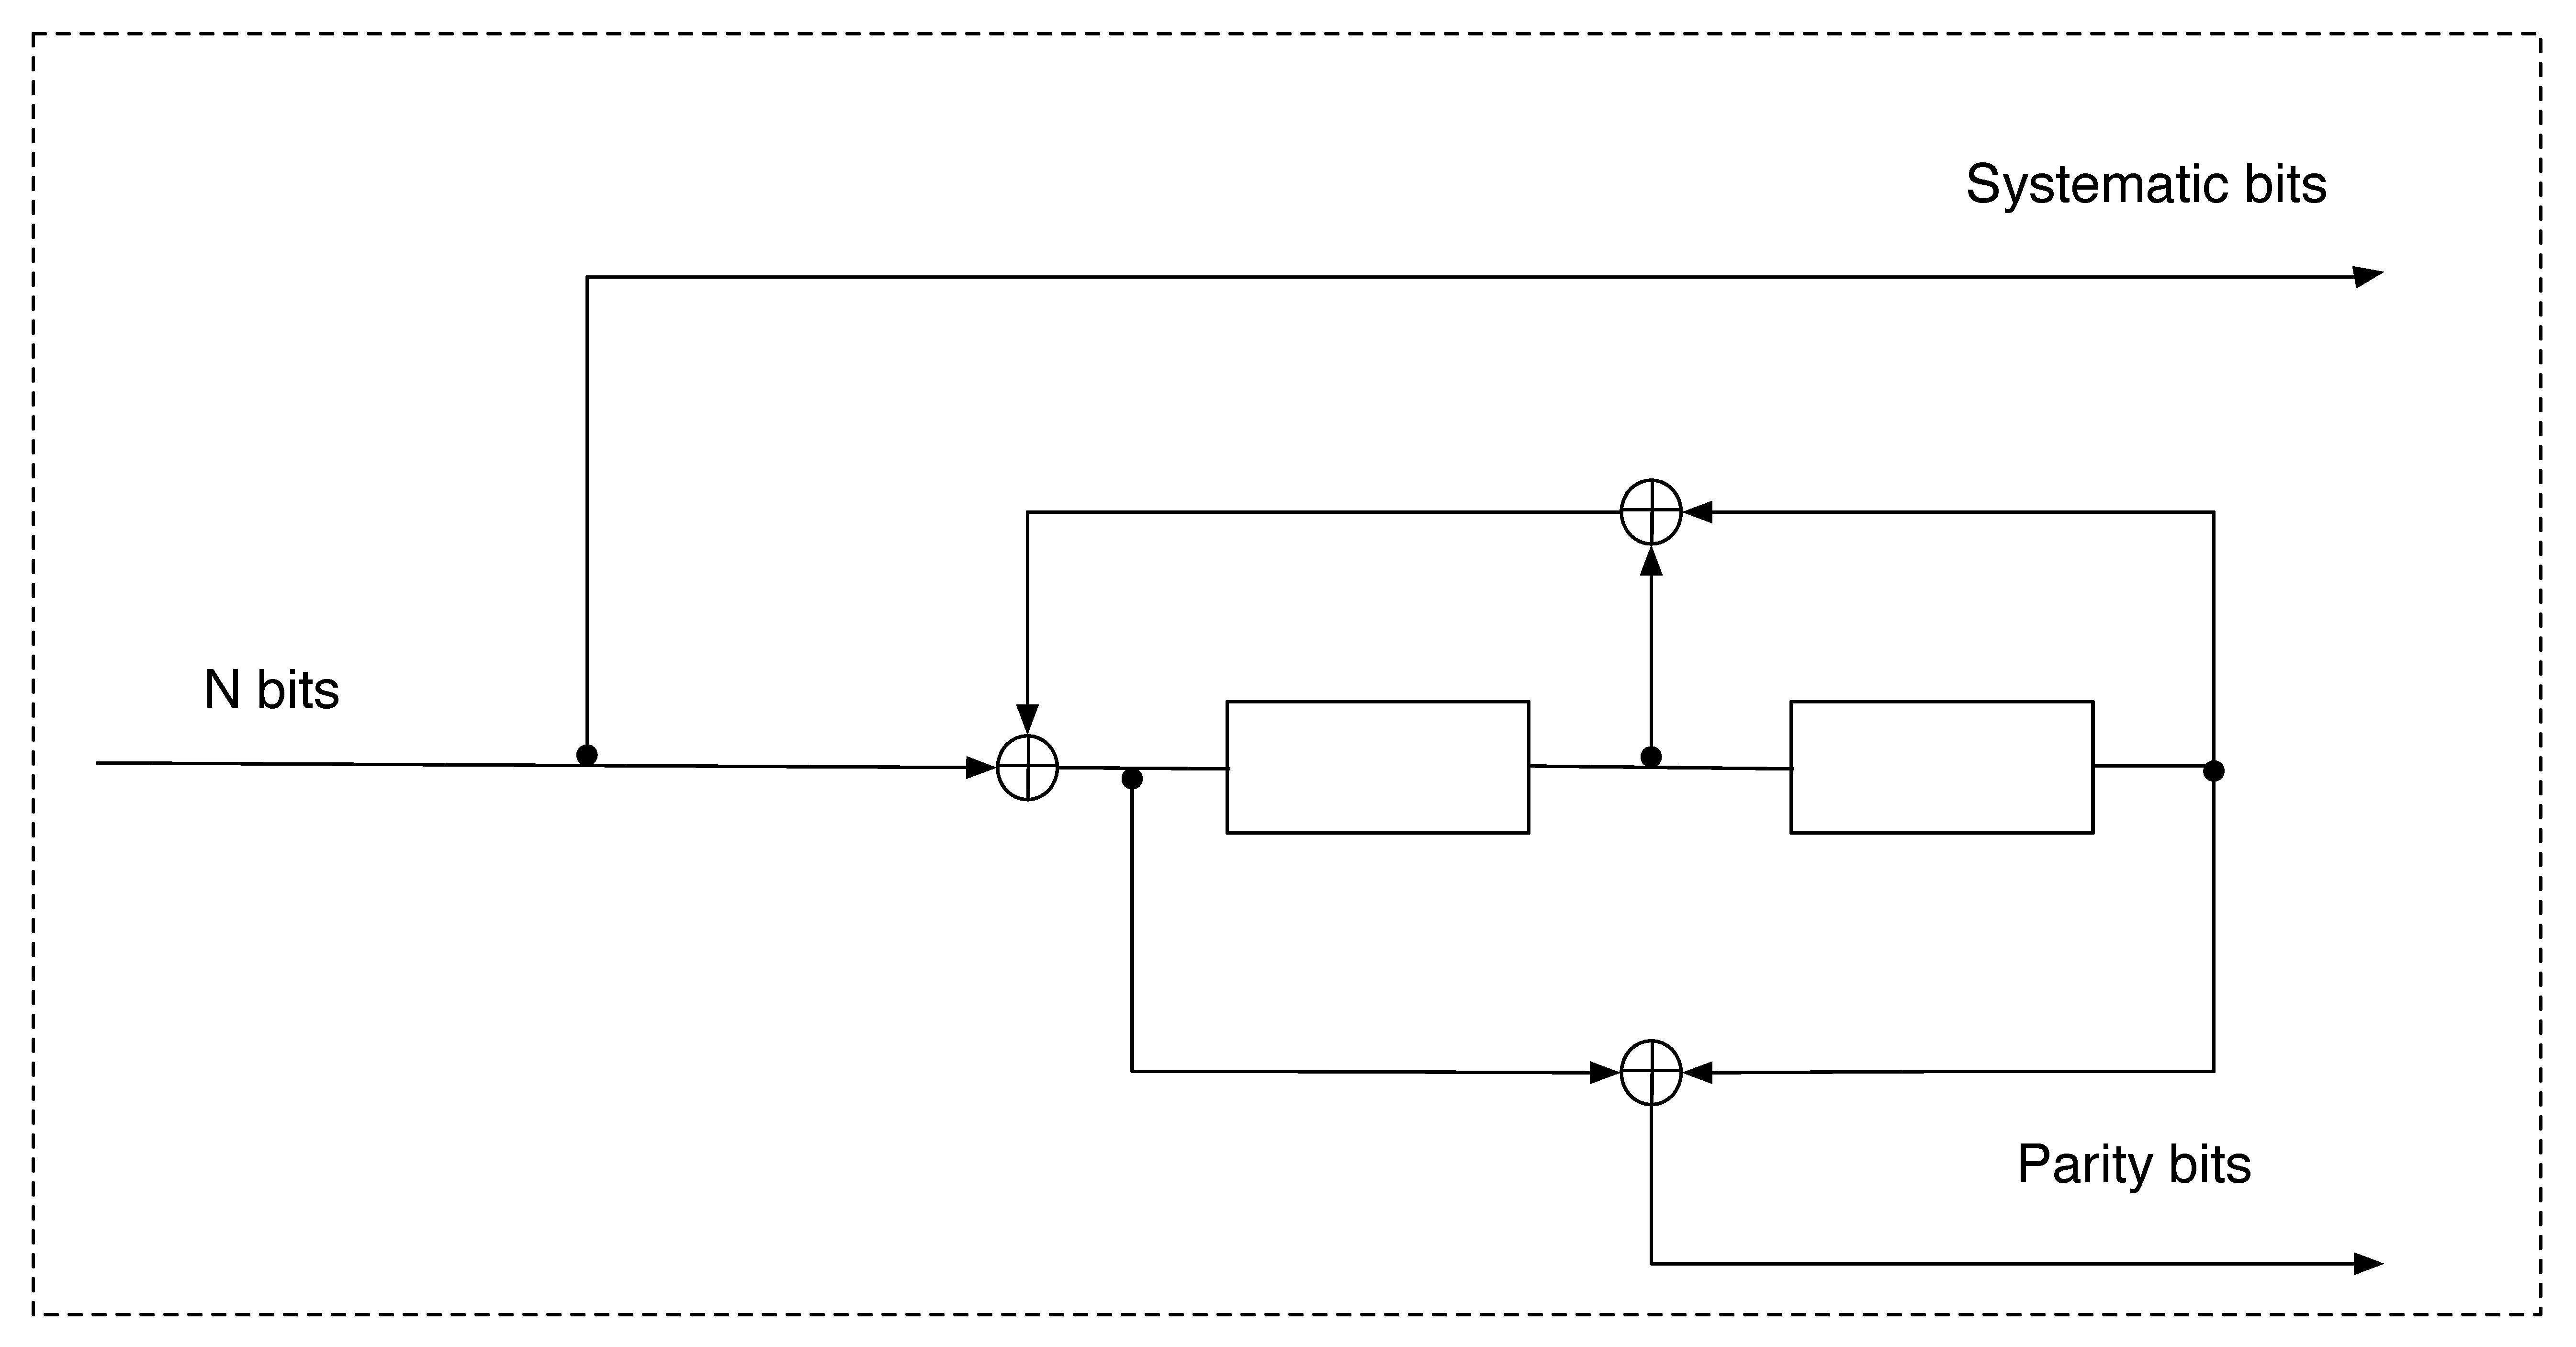
\includegraphics[width=0.45\textwidth]{./PaperSources/RSCExample3.pdf}
	%	\caption{$[\frac{1+x^2}{1+x+x^2}]$  RSC Encoder}
		%\label{fig1}
		%\end{figure}

%\begin{example}		
%An RSC encoder is shown in Figure \ref{fig1} with $k=1$ and $n=2$. Its parity generator\newline function is given by $[\frac{1+x^2}{1+x+x^2}]$, which may be written as $5/7$ in octal form, where $5 ~ \text{and} ~ 7$ correspond to the numerator and denominator of the generator function, respectively. 
 %For this RSC code, the cycle is $\bphi_g=\bphi_6 $ with a cycle length $\tau =3$. While $\bphi=(1~1~1~ 0~ 1~ 1~ 0~ 1~ 1~ 0~\cdots)$, which may be written in terms of the elements of GF(8) as $\bphi_7~\dot{\bphi_3}$ represents the impulse response. 
 %\end{example}
 % Moving forward all other examples and discussions relating to RSC codes will be done using the $5/7$ RSC code unless otherwise stated.

 %The knowledge of $\textbf{p}$ and $\tau$ will be used in deriving the method for determing which input messages generate low-weight parity bits. 